\section{Grundlagen}\label{kap:grundlagen}
In diesem Kapitel werden einige Grundlagen für die in Kapitel \ref{kap:featureextraktion} diskutierten Algorithmen besprochen.
\subsection{Was sind Sensordaten}\label{kap:sensordaten}

Um den Ablauf einer Maschine zu koordinieren und den aktuellen Zustand zu Überwachen werden oft Sensoren an den Maschinen angebracht. 
Diese Daten werden zu definierten Taktzeiten aufgenommen und weiterverarbeitet. 
Es kann sich dabei um einfache Kontaktsensoren handeln, mit einer begrenzten Anzahl an Zuständen oder um Sensoren mit einem reellen Zustandsbereich, wie Umgebungssensoren (Luftdruck-, Temperatursensor, etc.). 
In Abbildung\ \ref{fig:datasetoffice} sind Sensordaten in Form eines Datenplots dargestellt. 
Es handelt sich um Licht-, Temperatur- und Luftfeuchtigkeitssensordarten aus einem Büro im Zeitraum eines Arbeitstages. 
Abgebildet sind die Sensordaten zwischen $6:00$ Uhr und $19:00$Uhr.
\begin{figure}
    \centering
    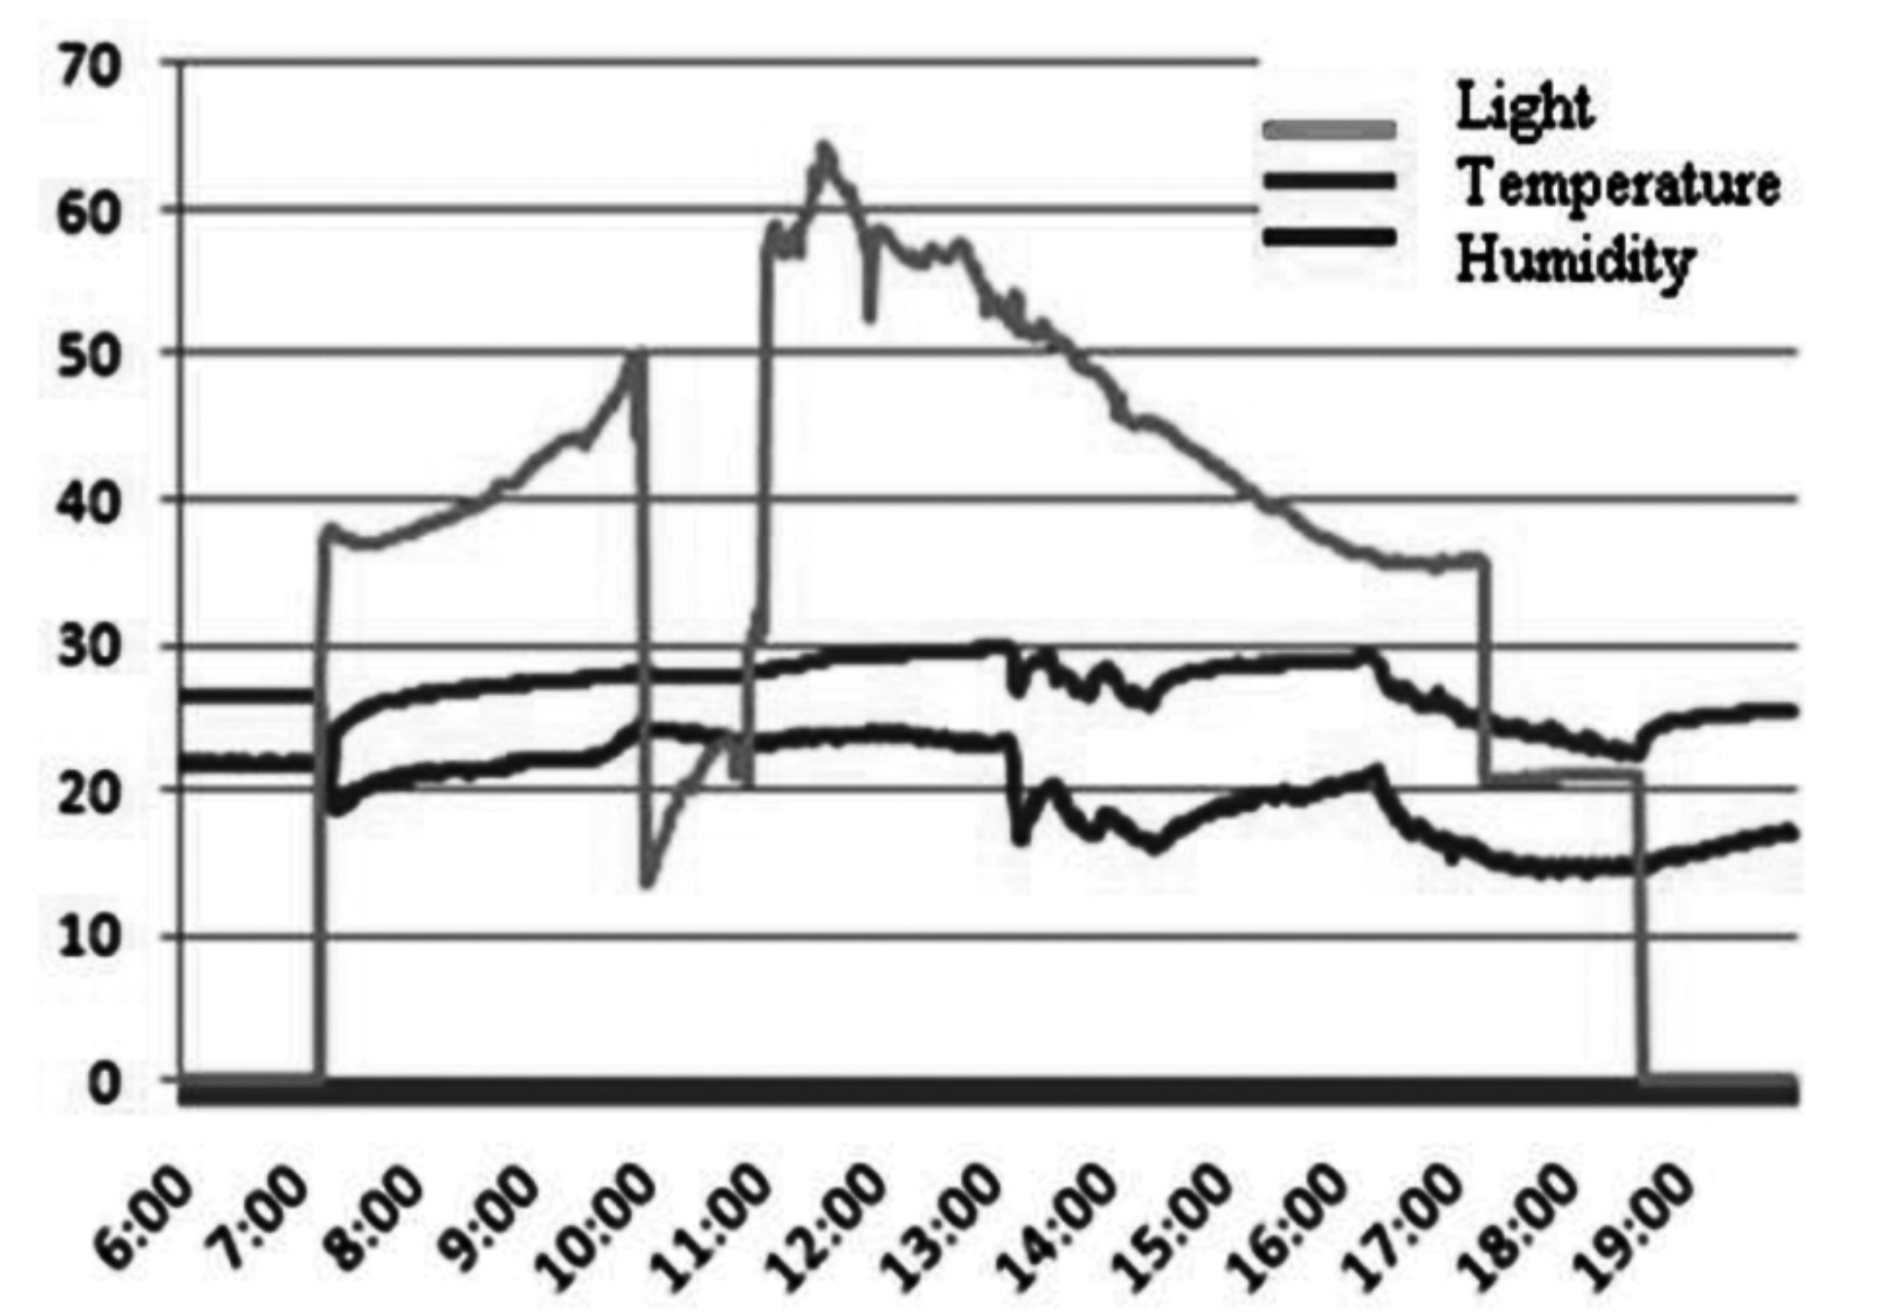
\includegraphics[width=.8\textwidth]{datasetOffice.png}
    \caption{Sensordatenabweichung anhand von Licht, Temperatur und Luftfeuchtigkeit im Buro innerhalb von einem Arbeitstag~\cite{moraru2010using}}
    \label{fig:datasetoffice}
\end{figure}

Um solche Sensordaten mathematisch weiterverarbeiten zu können, werden sie in Vektorform gebracht.
Ein Datensatz zum Zeitpunkt $6:00$ Uhr mit den Werten Licht = $0$, Temperatur=$22$ und Luftfeuchtigkeit = $25$ könnte dargestellt werden als:
\begin{equation}
    x_1 =
  \begin{pmatrix}
      0\\
      22\\
      25
  \end{pmatrix}
  \in \mathbb{R}^D
\end{equation}

Ein Vektor enthält somit einen Sensordatensatz zu einem Aufnahmezeitpunkt. Um Zeiträume darzustellen werden die Daten in eine Matrixform gebracht. Beispielsweise erhält man bei einer stündlichen Abtastrate und einem Zeitraum von $8:00$ Uhr bis $17:00$Uhr folgende Matrix:
\begin{equation}
    x_{1,10}
    \begin{pmatrix}
       38 & 40 & 46 & 24 & 60 & 58 & 51 & 44 & 40 & 36\\
       20 & 22 & 22 & 24 & 24 & 24 & 20 & 18 & 20 & 17\\
       25 & 28 & 28 & 28 & 29 & 30 & 20 & 27 & 29 & 26
    \end{pmatrix}
    \in \mathbb{R}^{D \times N}
\end{equation}

Diese mathematische Darstellung ist nur ein Beispiel und kann beliebig strukturiert werden.
Die erzeugte Matrix kann anschließend als Eingabe für Analysealgorithmen dienen.
Schon bei diesen geringen Datenmengen entsteht eine $D \times N $ große Matrix mit: 
\begin{itemize}
  \item $D=$ Anzahl der Paramter (Sensoren)
  \item $N=$ Anzahl der Daten.
\end{itemize}

Sollen auch noch Daten Raumübergreifend analysiert werden, können diese in Form eines Tensors dargestellt werden. Bei $M$ vielen Räumen entsteht ein $D \times N \times M$ großer Tensor.
Schon anhand dieses simplen Beispiels wird die Datenmenge und Komplexität der Daten ersichtlich.
In der Maschinenüberwachung entstehen dadurch schnell Datensätze im Millionenbereichen und da jede Komponente einer Maschine oft mit mehereren Sensoren ausgestattet ist, entstehen riesige Tensoren.

Neben klassischen Regressionsverfahren zur Datenanalyse, welche oft für Anomliedetektionen verwendet werden, gibt es auch verschiedene Klassifikationsverfahren. Dazu werden den Datensätzen manuell oder automatisiert Klassen hinzugefügt, welche jedem aufgenommenen Datenvektor eine Klasse zuordnet.

Mathematisch dargestellt erhalten wir dann einen Datensatz zum Zeitpunkt $t_1$ in Form eines Tupels $\tau_1=(t_1,x_1)$. Die für den Zeitpunkt definierten Merkmale sind dann in $x_k$ mit $(k=1_d)$ und $d \in D$. Diesem Tupel wird abhängig von den verwendeten Verfahren eine Klasse $y_1$ zugewiesen~\cite{gay2013feature}. Für den Zeitraum $(t_1,...,t_n)$ mit $n \in \mathbb{N}$ vielen Daten erhalten wir den Datensatz 
\begin{equation}
  K=\{ (\tau_{1_d},y_{1}), ... , (\tau_{n_d},y_n) \}
  \label{equ:trainingset}
\end{equation}
Das Ziel kann es sein das Tupel $(t_{n+1},y_{n+1})$ voherzusagen.

Es werden auch nicht nur feste Zeiträume betrachtet. 
Durch dauerhaft laufende Maschinen entstehen kontinuierliche Datenströme.
Daraus folgt ein kontiniuerlich wachsender Datenbestand.
Um ressourcenschonend und möglichst in Echtzeit die Daten zu analysieren, werden harte Speicher- und Laufzeitbedinungen an Analysealgorithmen gestellt.


\subsection{Feature Extraktion}\label{kap:featureextraktionuebersicht}
Im maschinellen Lernen werden im Wesentlichen zwei Methoden zur Datenanalyse betrachtet. Bei der \textbf{Regression} werden die Inputdaten auf Datenwerte reduziert ähnlich zur Approximation in Abbildung\ \ref{fig:FFETimeSeries}. Zu dem Bürodatensatz in Kapitel\ \ref{kap:sensordaten} könnte mithilfe von Regression die Anzahl an Mitarbeitern im Büro berechnet werden. In der \textbf{Klassifikation} werden Daten bestimmten Klassen zugeordnet. Im Gegensatz zur Regression würden nicht die Anzahl der Mitarbeiter, sondern Beispielsweise die Klassen \enquote{Büro besetzt} und \enquote{Büro unbesetzt} ausgegeben werden.

In beiden Verfahren ist die Grundlage der Entscheidung der Dateninput und die dazu gehörigen Parameter. Somit ist die Einhaltung der Algorithmenschranken abhängig von den Parametern $D$. Es gibt unterschiedliche Gründe, wesshalb versucht wird die Anzahl der Inputparamter anzupassen:
\begin{itemize}
  \setlength{\itemsep}{3pt}
  \renewcommand\labelitemi{\textbullet}
  \item Die Komplexität eines Lernalgorithmus hängt von der Anzahl an Eingabe Dimensionen $D$ und der Anzahl der Daten $N$ ab. Wird die Anzahl an Dimensionen und somit Paramtern reudziert, dann reduziert sich auch die Komplexität~\cite{alpaydin2014introduction}.
  \item Wenn die richtigen Parameter ausgewählt werden, sind die Algorithmen teilweise sogar stabiler~\cite{morchen2003time}
  \item Wenn eine Eingabe keinen Einfluss auf die Funktion und das Ergebnis des Algorithmus hat, können diese Kosten eingespart werden~\cite{alpaydin2014introduction}.
  \item Modelle aus Lernalgorithmen sind oft auf kleine Datensätze robuster, da diese eine geringere Variance und Rauschen aufweisen~\cite{alpaydin2014introduction}.
  \item Wenn Daten durch weniger Merkmale beschrieben werden könne, bekommt der Mensch ein besseres Verständnis über den gesamten Prozess~\cite{alpaydin2014introduction}.
  \item Je weniger Dimensionen, desto leichter die Visualisierung~\cite{alpaydin2014introduction}.
\end{itemize}

Aus diesen Gründen wird versucht die Anzahl der Eingabeparameter in einen Algorithmus möglichst zu reduzieren. Um so eine Dimensionsreduktion zu erreichen gibt es zweit Hauptansätze:
\paragraph{Feature Selektion} ist ein Ansatz, indem die Dimension $D$ auf eine Dimension $L$ reduziert wird. Dabei werden interessante Parameter aus der Parametermenge entnommen und die restlichen $D-L$ Parameter werden verworfen. \enquote{Features} sind dabei Merkmale, wodurch sich Daten unterscheiden lassen. In diesem Ansatz sind die Merkmale direkt die ausgewählten Eingabeparameter~\cite{alpaydin2014introduction}.

\paragraph{Feature Extraktion} dagegen entnimmt nicht vorhandene Eingabeparameter sondern geniert bzw. extrahiert aus den vorhandenen Parameter neue Merkmale. Die Anzahl an Merkmalen ergibt die neue Dimension $L$ ~\cite{alpaydin2014introduction}.
Merkmale können einfache, auf die Parameter angewedete, Funktionen sein, wie in Abbildung\ \ref{fig:FFETimeSeries} der Durchschnitt und die Steigung im Merkmalsraum (d). Oder komplexere Parameterkombinationen in höher Dimensionalenräumen, wie Verlaufsmuster von Raumflächen.

Auf Lernalgorithmen angewendet ist es letztlich immer das Ziel die Features so zu wählen und zu parametrisieren, dass der ermittelte Wert oder die ermittelten Zuordnung aus einem Lernalgorithmus dem tatsächlichen möglichst ähneln. Formal beschrieben anhand dem Datensatz \ref{equ:trainingset}. Sei $p(x_i)$ die Funktion, welche das Ergebnis des gewählten Algorithmus und des Trainingsdatensatzes ist. Es soll versucht werden den Fehlerunterschied

\begin{equation}
  \sigma = p(x_i)-y_i
\end{equation}

möglichst zu reduzieren~\cite{gensler2015fast}. Die konkreten Herausforderungen und Herangehensweisen in der Maschinenüberwachung werden in dem folgenden Kapitel besprochen
